%%%%%%%%%%%%%%%%%%%%%%%%%%%%%%%%%%%%%%%%%
% Beamer Presentation
% LaTeX Template
% Version 2.0 (March 8, 2022)
%
% This template originates from:
% https://www.LaTeXTemplates.com
%
% Author:
% Vel (vel@latextemplates.com)
%
% License:
% CC BY-NC-SA 4.0 (https://creativecommons.org/licenses/by-nc-sa/4.0/)
%
%%%%%%%%%%%%%%%%%%%%%%%%%%%%%%%%%%%%%%%%%

%----------------------------------------------------------------------------------------
%	PACKAGES AND OTHER DOCUMENT CONFIGURATIONS
%----------------------------------------------------------------------------------------

\documentclass[
	11pt, % Set the default font size, options include: 8pt, 9pt, 10pt, 11pt, 12pt, 14pt, 17pt, 20pt
	%t, % Uncomment to vertically align all slide content to the top of the slide, rather than the default centered
	%aspectratio=169, % Uncomment to set the aspect ratio to a 16:9 ratio which matches the aspect ratio of 1080p and 4K screens and projectors
]{beamer}

\graphicspath{{Images/}{./}} % Specifies where to look for included images (trailing slash required)

\usepackage{booktabs} % Allows the use of \toprule, \midrule and \bottomrule for better rules in tables
\usepackage[spanish]{babel}
%----------------------------------------------------------------------------------------
%	SELECT LAYOUT THEME
%----------------------------------------------------------------------------------------

% Beamer comes with a number of default layout themes which change the colors and layouts of slides. Below is a list of all themes available, uncomment each in turn to see what they look like.

%\usetheme{default}
%\usetheme{AnnArbor}
%\usetheme{Antibes}
%\usetheme{Bergen}
%\usetheme{Berkeley}
%\usetheme{Berlin}
\usetheme{Boadilla} %me gusta
%\usetheme{CambridgeUS}
%\usetheme{Copenhagen}
%\usetheme{Darmstadt}
%\usetheme{Dresden}
%\usetheme{Frankfurt}
%\usetheme{Goettingen} %dos dos
%\usetheme{Hannover} %dos dos
%\usetheme{Ilmenau}
%\usetheme{JuanLesPins}
%\usetheme{Luebeck}
%\usetheme{Madrid}
%\usetheme{Malmoe}
%\usetheme{Marburg}
%\usetheme{Montpellier}
%\usetheme{PaloAlto}
%\usetheme{Pittsburgh}
%\usetheme{Rochester} %muy flat
%\usetheme{Singapore}
%\usetheme{Szeged}
%\usetheme{Warsaw}

%----------------------------------------------------------------------------------------
%	SELECT COLOR THEME
%----------------------------------------------------------------------------------------

% Beamer comes with a number of color themes that can be applied to any layout theme to change its colors. Uncomment each of these in turn to see how they change the colors of your selected layout theme.

%\usecolortheme{albatross}
%\usecolortheme{beaver}
%\usecolortheme{beetle}
%\usecolortheme{crane}
%\usecolortheme{dolphin}
%\usecolortheme{dove}
%\usecolortheme{fly}
%\usecolortheme{lily} %default
%\usecolortheme{monarca}
%\usecolortheme{seagull}
%\usecolortheme{seahorse}
%\usecolortheme{spruce}
%\usecolortheme{whale}
%\usecolortheme{wolverine}

%----------------------------------------------------------------------------------------
%	SELECT FONT THEME & FONTS
%----------------------------------------------------------------------------------------

% Beamer comes with several font themes to easily change the fonts used in various parts of the presentation. Review the comments beside each one to decide if you would like to use it. Note that additional options can be specified for several of these font themes, consult the beamer documentation for more information.

\usefonttheme{default} % Typeset using the default sans serif font
%\usefonttheme{serif} % Typeset using the default serif font (make sure a sans font isn't being set as the default font if you use this option!)
%\usefonttheme{structurebold} % Typeset important structure text (titles, headlines, footlines, sidebar, etc) in bold
%\usefonttheme{structureitalicserif} % Typeset important structure text (titles, headlines, footlines, sidebar, etc) in italic serif
%\usefonttheme{structuresmallcapsserif} % Typeset important structure text (titles, headlines, footlines, sidebar, etc) in small caps serif

%------------------------------------------------

%\usepackage{mathptmx} % Use the Times font for serif text
\usepackage{palatino} % Use the Palatino font for serif text

\usepackage[ruled,vlined]{algorithm2e}
%\usepackage{helvet} % Use the Helvetica font for sans serif text
\usepackage[default]{opensans} % Use the Open Sans font for sans serif text
%\usepackage[default]{FiraSans} % Use the Fira Sans font for sans serif text
%\usepackage[default]{lato} % Use the Lato font for sans serif text
\usepackage{biblatex}
%----------------------------------------------------------------------------------------
%	SELECT INNER THEME
%----------------------------------------------------------------------------------------

% Inner themes change the styling of internal slide elements, for example: bullet points, blocks, bibliography entries, title pages, theorems, etc. Uncomment each theme in turn to see what changes it makes to your presentation.

%\useinnertheme{default}
\useinnertheme{circles}
%\useinnertheme{rectangles}
%\useinnertheme{rounded}
%\useinnertheme{inmargin}

%----------------------------------------------------------------------------------------
%	SELECT OUTER THEME
%----------------------------------------------------------------------------------------

% Outer themes change the overall layout of slides, such as: header and footer lines, sidebars and slide titles. Uncomment each theme in turn to see what changes it makes to your presentation.

%\useoutertheme{default}
%\useoutertheme{infolines}
%\useoutertheme{miniframes}
%\useoutertheme{smoothbars}
%\useoutertheme{sidebar}
%\useoutertheme{split}
%\useoutertheme{shadow}
%\useoutertheme{tree}
%\useoutertheme{smoothtree}

%\setbeamertemplate{footline} % Uncomment this line to remove the footer line in all slides
%\setbeamertemplate{footline}[page number] % Uncomment this line to replace the footer line in all slides with a simple slide count

%\setbeamertemplate{navigation symbols}{} % Uncomment this line to remove the navigation symbols from the bottom of all slides

%----------------------------------------------------------------------------------------
%	PRESENTATION INFORMATION
%----------------------------------------------------------------------------------------

\title[Inteligencia Computacional]{Lógica Difusa para el control de una intersección} % The short title in the optional parameter appears at the bottom of every slide, the full title in the main parameter is only on the title page

%\subtitle{Optional Subtitle} % Presentation subtitle, remove this command if a subtitle isn't required

\author[Luis Ballado]{Luis Ballado} % Presenter name(s), the optional parameter can contain a shortened version to appear on the bottom of every slide, while the main parameter will appear on the title slide

\institute[CINVESTAV]{CINVESTAV - UNIDAD TAMAULIPAS \\ \smallskip \textit{luis.ballado@cinvestav.mx}} % Your institution, the optional parameter can be used for the institution shorthand and will appear on the bottom of every slide after author names, while the required parameter is used on the title slide and can include your email address or additional information on separate lines

\date[\today]{\today} % Presentation date or conference/meeting name, the optional parameter can contain a shortened version to appear on the bottom of every slide, while the required parameter value is output to the title slide

%----------------------------------------------------------------------------------------

\begin{document}

%----------------------------------------------------------------------------------------
%	TITLE SLIDE
%----------------------------------------------------------------------------------------

\begin{frame}
	\titlepage % Output the title slide, automatically created using the text entered in the PRESENTATION INFORMATION block above
\end{frame}

%----------------------------------------------------------------------------------------
%	TABLE OF CONTENTS SLIDE
%----------------------------------------------------------------------------------------

% The table of contents outputs the sections and subsections that appear in your presentation, specified with the standard \section and \subsection commands. You may either display all sections and subsections on one slide with \tableofcontents, or display each section at a time on subsequent slides with \tableofcontents[pausesections]. The latter is useful if you want to step through each section and mention what you will discuss.

\begin{frame}
	\frametitle{Contenido} % Slide title, remove this command for no title
	
	\tableofcontents % Output the table of contents (all sections on one slide)
	%\tableofcontents[pausesections] % Output the table of contents (break sections up across separate slides)
\end{frame}

%----------------------------------------------------------------------------------------
%	PRESENTATION BODY SLIDES
%----------------------------------------------------------------------------------------

\section{Introducción} % Sections are added in order to organize your presentation into discrete blocks, all sections and subsections are automatically output to the table of contents as an overview of the talk but NOT output in the presentation as separate slides

%------------------------------------------------

\begin{frame}
  \frametitle{Introducción}
  
  {\footnotesize CDMX no es la ciudad de México con más tráfico: Monterrey entra al top 10 de las ciudades más congestionadas del mundo} \footcite{xataka}
  \begin{figure}
    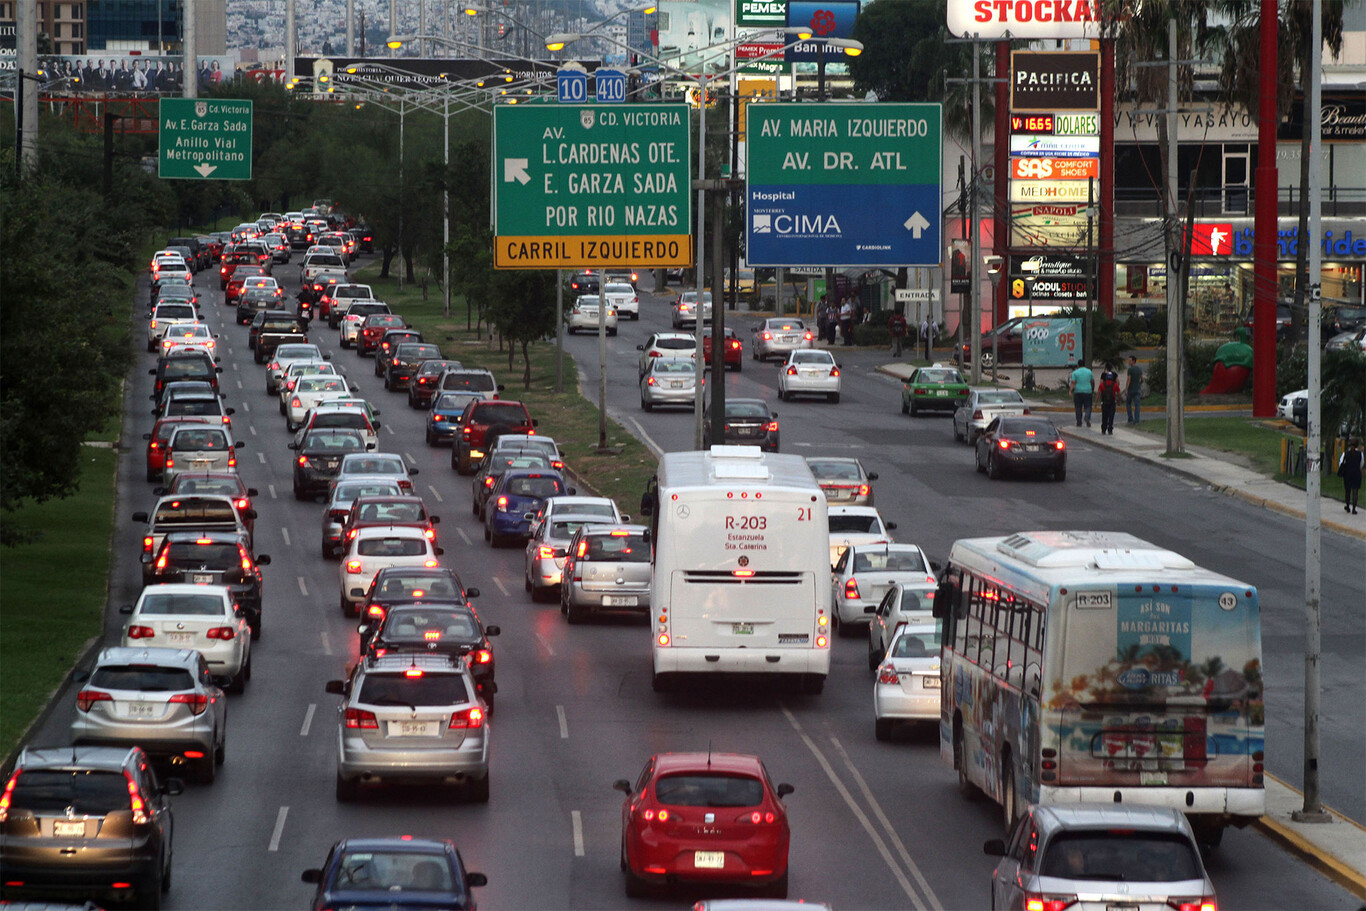
\includegraphics[width=0.6\linewidth]{trafico.jpeg}
    \caption{Av Lázaro Cárdenas San Pedro Garza García, N.L.}
  \end{figure}
  
\end{frame}

\begin{frame}
  \frametitle{¿Cuánto cuesta la congestión vehicular en México?}
             {\footnotesize La congestión de vehículos cuesta tiempo, calidad de vida, desarrollo económico.} \footcite{imco}
             
  \begin{figure}
    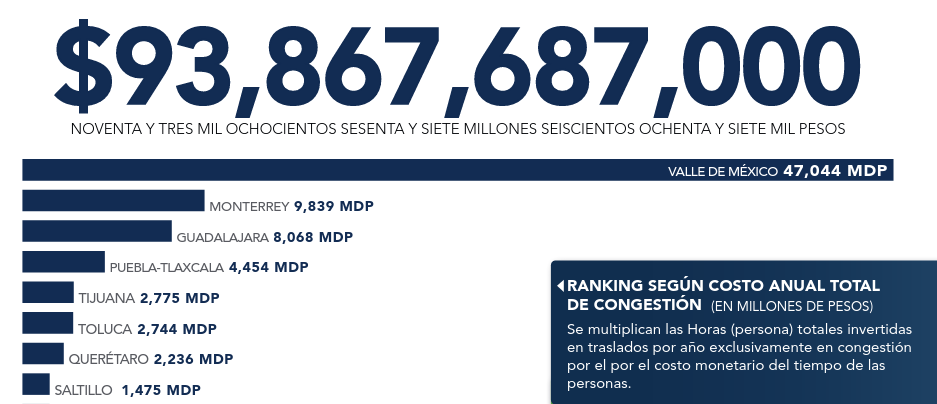
\includegraphics[width=0.9\linewidth]{costo_movilidad.png}
  \end{figure}
  
\end{frame}

\begin{frame}
  \frametitle{Evolución de los semáforos}
  \bigskip % Vertical whitespace

  El origen de los semáforos para el control de tráfico vehicular se remonta al año \textbf{1868} en la ciudad de Londres, donde se instaló el primer semáforo. \\

  \begin{figure}
    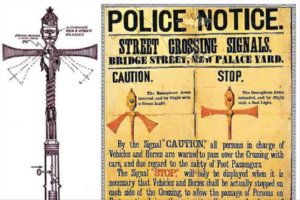
\includegraphics[width=0.3\linewidth]{primer_semaforo.png}
  \end{figure}
  
  Para el año \textbf{1920}, se agregó la luz ámbar intermedia para advertir del cambio de luces y así evitar muchos accidentes de tránsito.\\
\end{frame}

\begin{frame}
  \bigskip % Vertical whitespace
  En México, el presidente Porfirio Díaz estableció un cuerpo de policias de tránsito para regular el flujo vehicular en las principales avenidas; fué hasta \textbf{1932} que se instaló el primer semáforo en el cruce de Ave. Juárez y San Juan Letrán. \footcite{tesis}

  \begin{figure}
    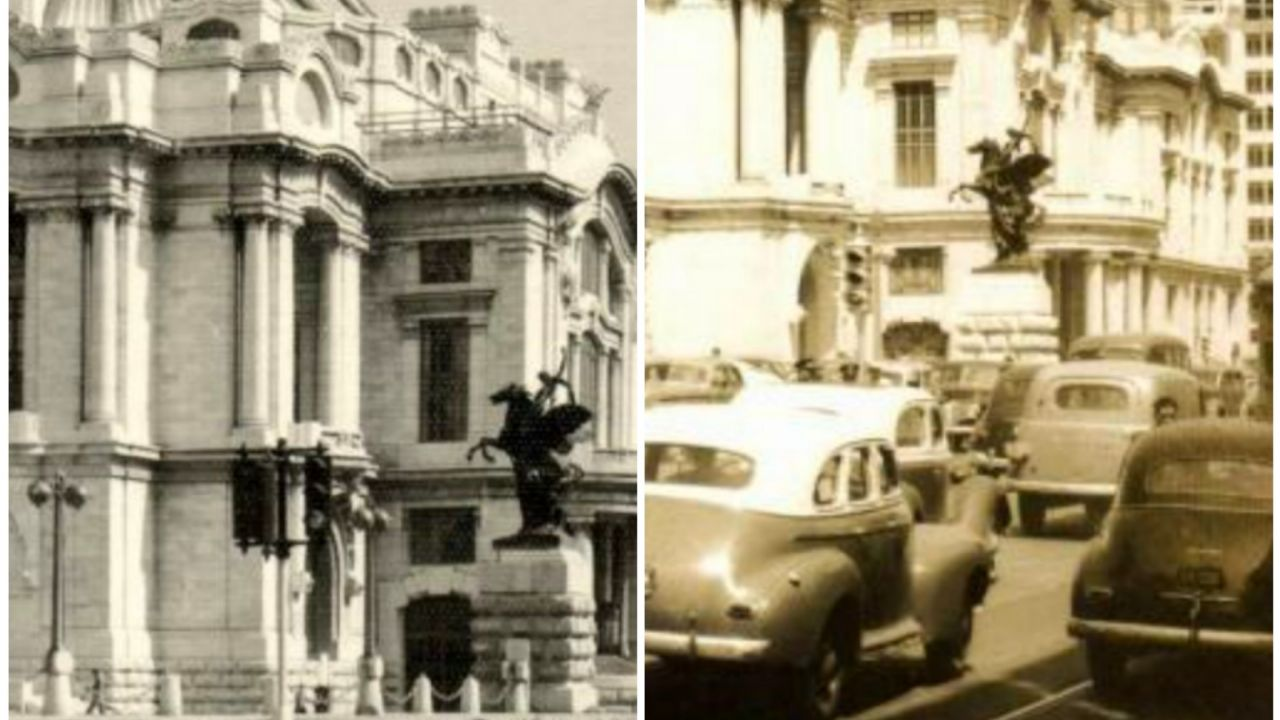
\includegraphics[width=0.5\linewidth]{primer_semaforo_mex.jpg}
  \end{figure}
  
\end{frame}
\begin{frame}
  A partir de la invención de los semáforos electrónicos de tres luces, se presentó la necesidad de automatizar los mecanismos de control, como respuesta a esta necesidad surgieron los semáforos cronometrados o de temporizador con intervalos fijos.\\

  Actualmente, los semaforos funcionan mediante diodos LED, y se han añadido extensiones para peatones.

  \begin{figure}
    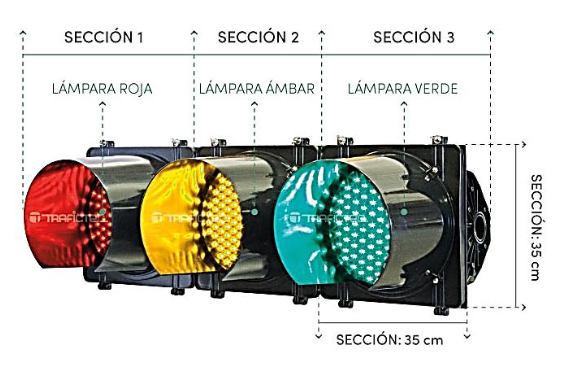
\includegraphics[width=0.5\linewidth]{semaforos.png}
  \end{figure}
  
\end{frame}

\begin{frame}
  \frametitle{Clasificación de los semáforos}
  
  En México el Manual de Señalización Vial y Dispositivos de seguridad (Secretaría de Comunicaciones y Transportes, 2014) establece los siguientes criterios para la clasificación de semáforos para el control del tránsito de vehículos. \footcite{tesis}
  \bigskip % Vertical whitespace

  \begin{itemize}
  \item Semáforos no accionados por el tránsito
  \item Control sin mecanismo de sincronización para intersecciones aisladas
  \item Control con mecanismo de sincronización para intersecciones aisladas
  \item Control que permite coordinación para intersecciones sucesivas
  \end{itemize}

\end{frame}

\begin{frame}

  \begin{itemize}
  \item Semáforos accionados por el tránsito
  \item Control parcialmente accionado por el tránsito
  \item Control totalmente accionado por el tránsito
  \item Control adaptable al tránsito
  \end{itemize}
\end{frame}

\section{Propuesta}
\begin{frame}
  \frametitle{Propuesta}

  Tener un acercamiento a un ecosistema de simulación de tráfico, que me permita simular flujo de vehículos y poder controlar el entorno, capaz de pensar en integraciones sencillas con tecnología a nuestro alcance. 

  \begin{figure}
    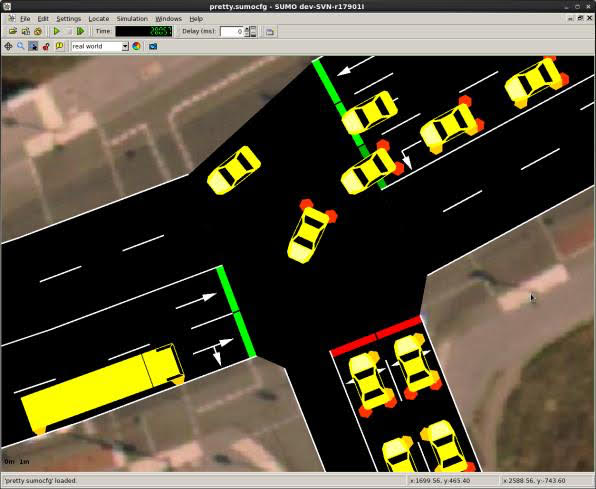
\includegraphics[width=0.5\linewidth]{sumo.jpg}
  \end{figure}
  
\end{frame}

\section{Trabajo previo}
\begin{frame}
  \frametitle{Trabajo previo}

  Ya que el control de tráfico es un problema muy común en todas partes del mundo, el trabajo ó productos terminados son variados, mencionando algunos de los actualmente existentes.\\
\bigskip % Vertical whitespace
  El funcionamiento de los semáforos tradicionales no es muy eficiente. Paran independientemente de cuál sea la situación. Aunque vengan 30 coches de una dirección y ninguno de la otra, los 30 coches tendrán que parar a esperar a que se ponga en verde. Esto, en cambio, podría cambiar mediante la Inteligencia Artificial. Y no es algo lejano, sino que algunos gobiernos, como el londinense, ya lo están probando. \footcite{infobae}\\
  
\end{frame}

\begin{frame}
  
  \begin{figure}
    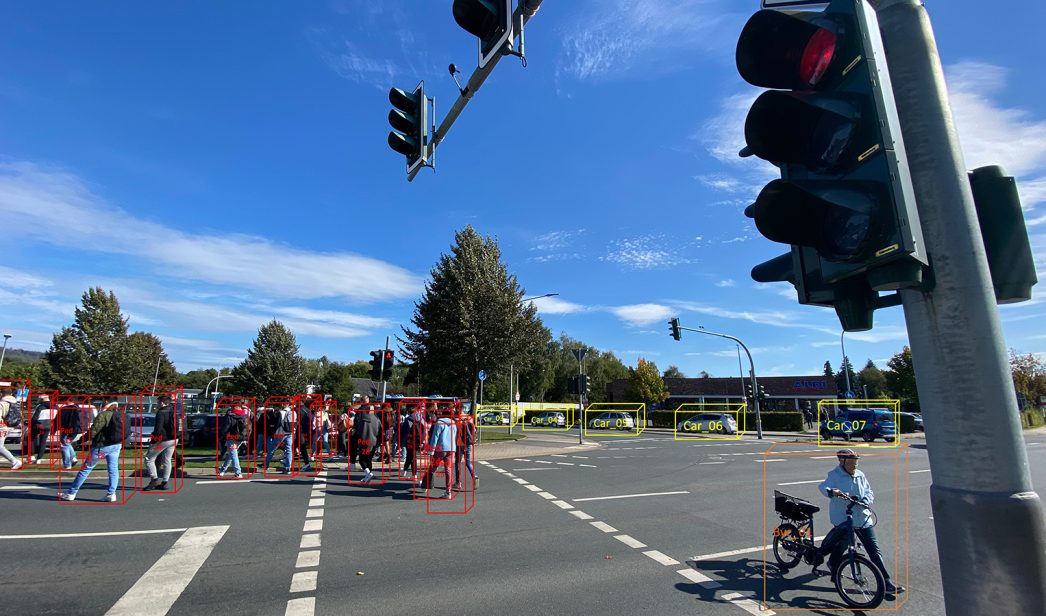
\includegraphics[width=0.7\linewidth]{interseccion_ia.jpg}
  \end{figure}
  
    
\end{frame}

\begin{frame}
  
  \begin{figure}
    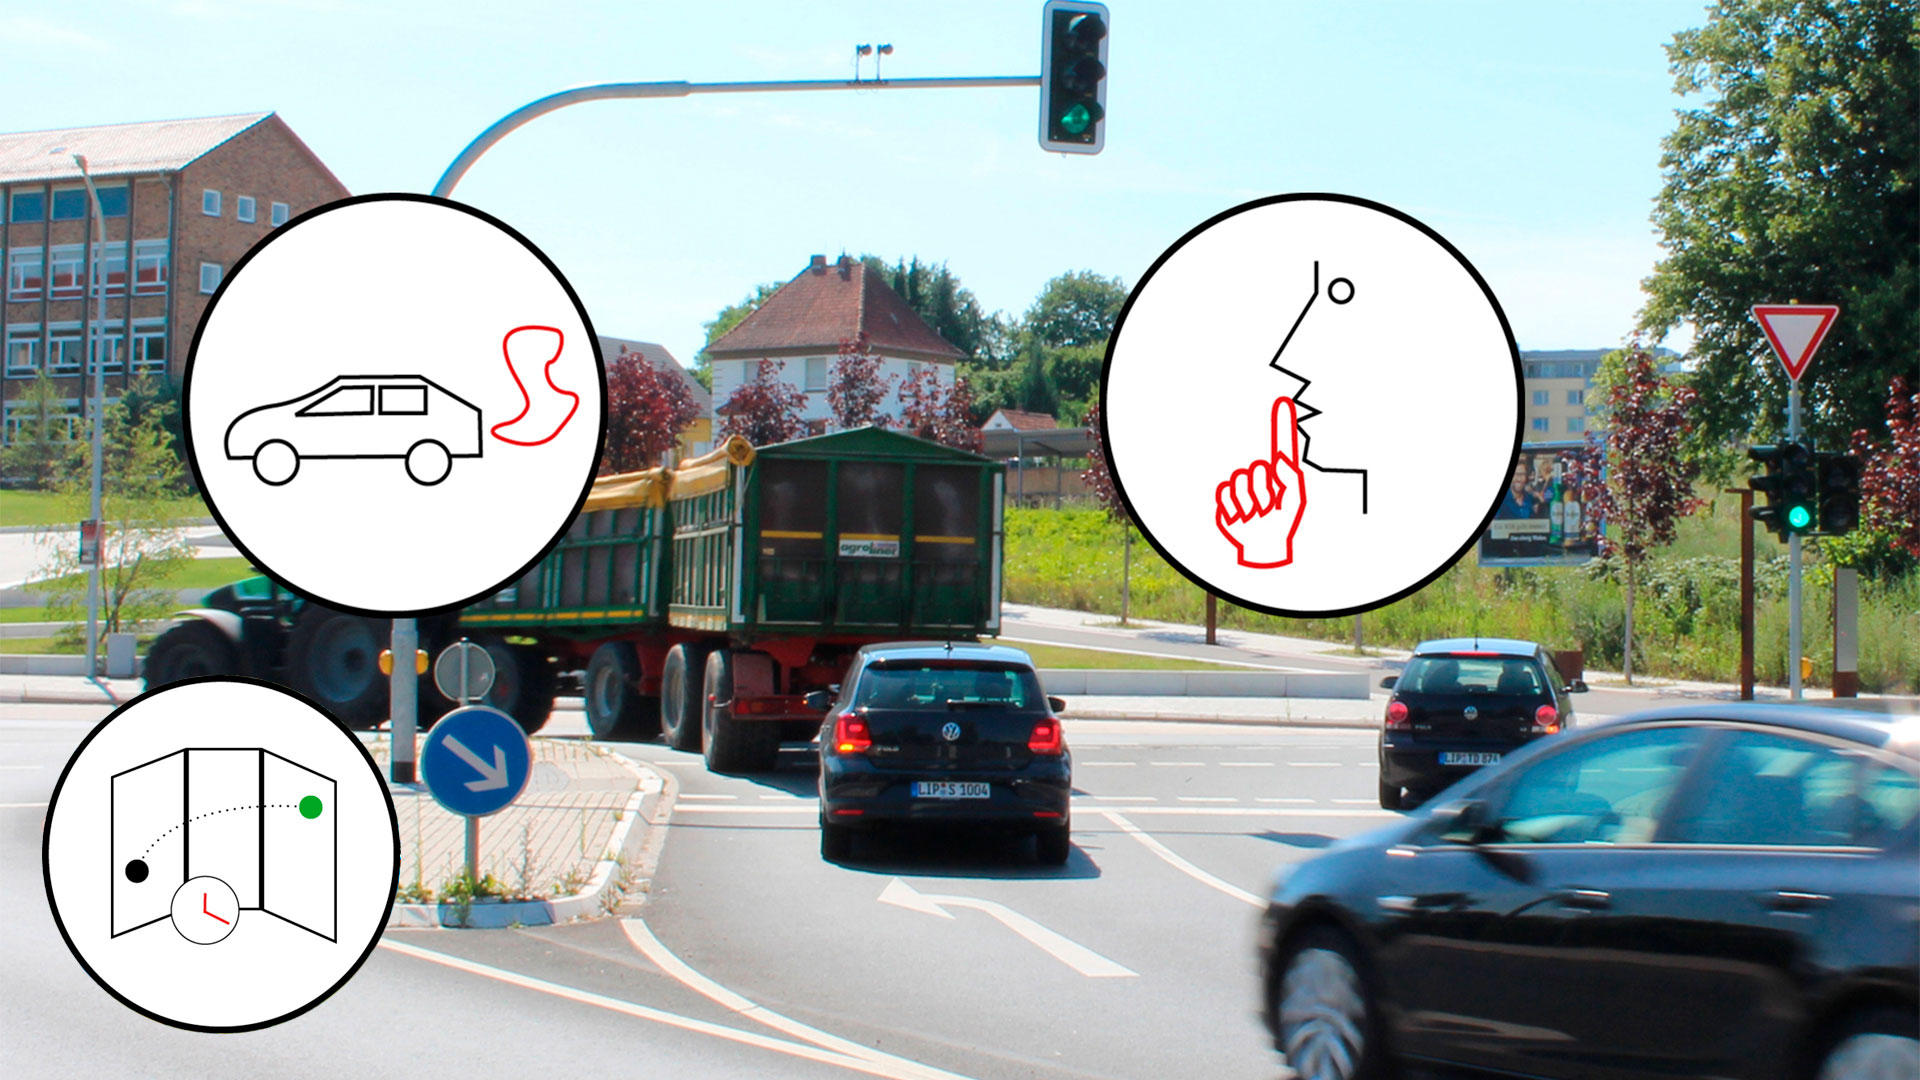
\includegraphics[width=0.8\linewidth]{sem_int.jpg}
  \end{figure}
  
    
\end{frame}

\begin{frame}
  \begin{figure}
    
\includegraphics[width=0.8\linewidth]{audi.jpg}\footcite{audi}
  \end{figure}
\end{frame}

\begin{frame}
  
  \begin{figure}
    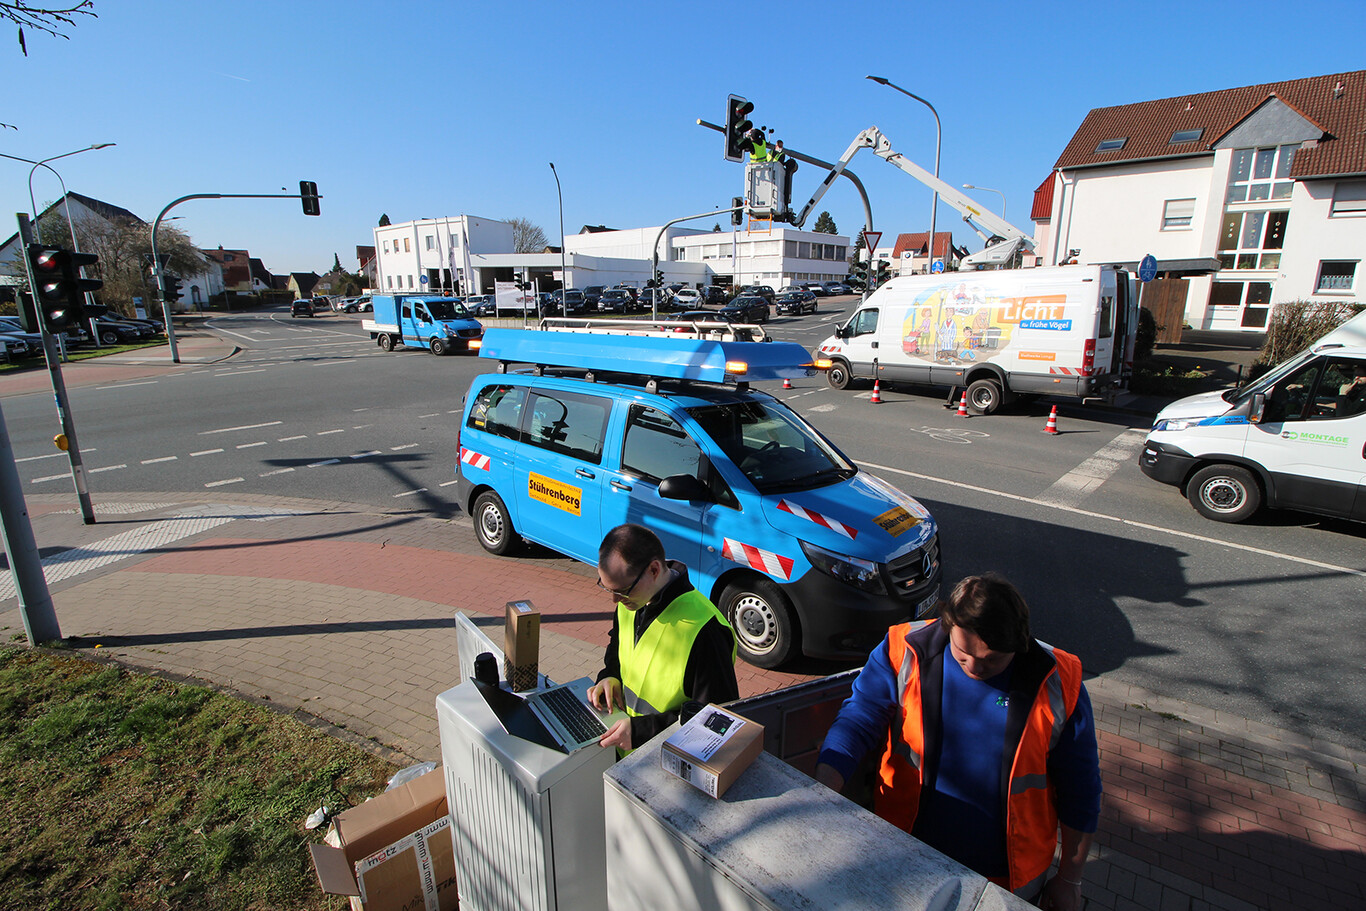
\includegraphics[width=0.8\linewidth]{street_code.jpeg}
  \end{figure}
  
    
\end{frame}
%------------------------------------------------

\section{Descripción de la propuesta}
\begin{frame}
  \frametitle{Solución propuesta}
  
  Recordemos que la lógica difusa trabaja para aquellos problemas dónde la complejidad de sus variables y manipulaciones son muy altas. \\

  No podemos usar algoritmos geneticos, ni redes neuronales porque el problema se volveria incalculable en un tiempo de espera corto. Volviendo nuestro problema -NP- tiempo no polinomial. No es lo que buscamos, queremos una solución muy rápida y ágil para este problema.\\
  \bigskip % Vertical whitespace
  \begin{center}
    LÓGICA DIFUSA $\implies$ LÓGICA DEL HOMBRE
  \end{center}
      
\end{frame}

\begin{frame}
  \begin{figure}
    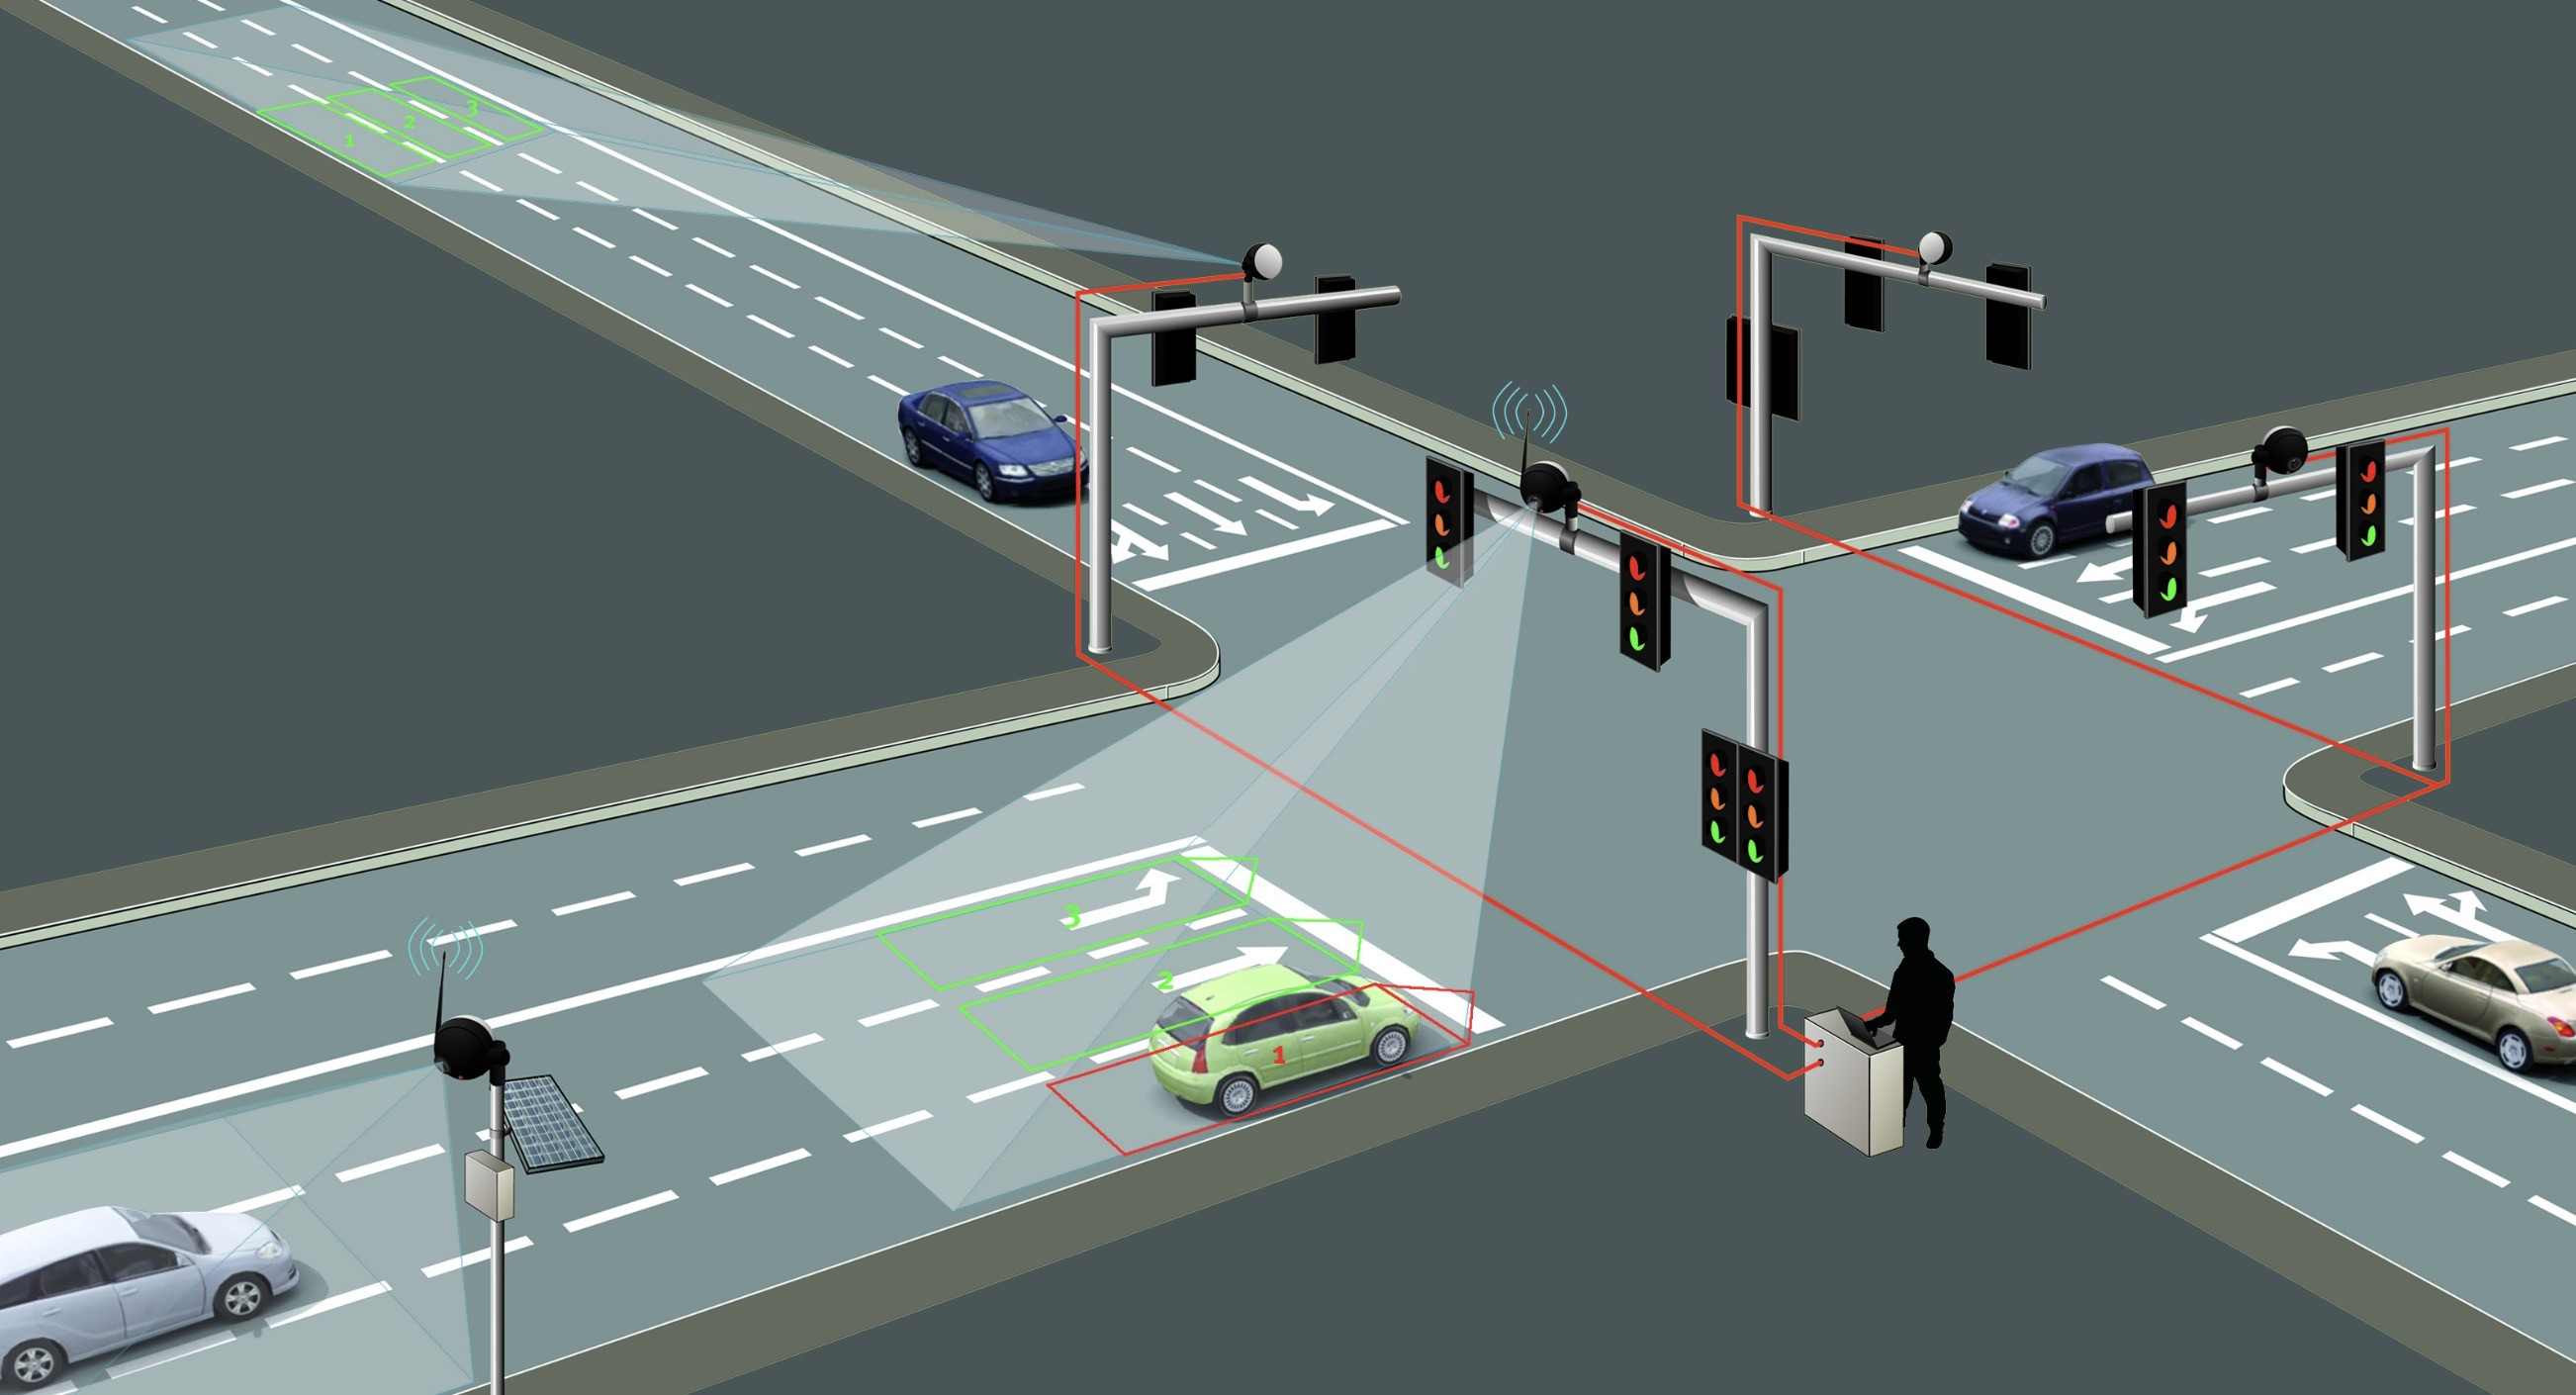
\includegraphics[width=0.8\linewidth]{control_systems.jpg}\footcite{autoevolucion}\\
  \end{figure}
\end{frame}

\begin{frame}
  \frametitle{Arquitectura de un sistema de lógica difusa}

  \begin{enumerate}
  \item Módulo de Fuzzificación: Transformar las señales de entrada (crisp) en conjuntos borrosos.
  \item Conocimientos: Reglas del experto (IF-THEN rules)
  \item Máquina de Inferencia: Simula el razonamiento humano haiendo una inferencia de la entrada y las reglas del experto.
  \item Defuzzificación: Transformar los conjuntos difusos obtenidos por la máquina de inferencia a valores realies (crips).
  \end{enumerate}

  Funciones de membresia.
  \begin{itemize}
  \item eje x - representa el universo de discurso
  \item eje y - representa el grado de pertenencia en el intervalo [0,1]
  \end{itemize}
  
\end{frame}

\begin{frame}
  Partiendo de lo anterior,

  \begin{enumerate}
  \item Identificar las variables de entrada:
    
    \begin{itemize}
    \item número de vehiculos esperando en cada intersección
    \item tiempo desde la última vez que el semaforo tuvo un verde
    \end{itemize}

  \item Identificar las variables de salida: en nuestro caso será la duración de la luz verde en cada intersección

  \item Determinar los conjuntos difusos: los conjuntos difusos pueden ser identificados analizando las variables de entrada y los rangos para cada variable
  \end{enumerate}
\end{frame}

\begin{frame}
  \begin{figure}
    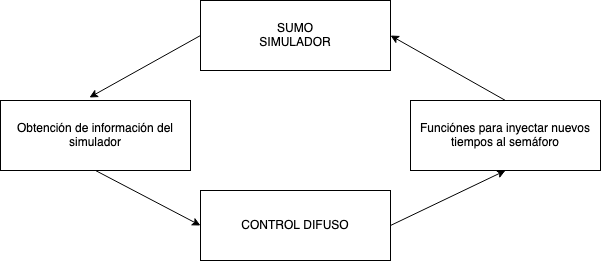
\includegraphics[width=0.9
      \linewidth]{diagrama_sumo.png}
    \caption{Diagrama solución en simulador}
  \end{figure}
\end{frame}

\section{DEMO}
\begin{frame}
  \begin{center}
    CORRAMOS LA DEMOSTRACIÓN
  \end{center}
\end{frame}

\begin{frame}{REFERENCIAS}
  \begin{thebibliography}{10}
    \setbeamertemplate{bibliography item}[text]
  \bibitem{xakata}
    XAKATA, "CDMX no es la ciudad de México con más tráfico", \url{https://www.xataka.com.mx/automovil/ciudad-mexicana-trafico-no-cdmx-monterrey-10-congestionadas-mundo}, Enero 2023.
  \bibitem{imco}
    Instituto Mexicano para la Competitividad A.C., "¿Cuánto cuesta la congestión en México?", \url{https://www.xataka.com.mx/automovil/ciudad-mexicana-trafico-no-cdmx-monterrey-10-congestionadas-mundo}, 2018.
  \bibitem{infobae}
    Infobae, "Sistema de semáforos inteligentes con IA", \url{https://www.infobae.com/autos/2022/03/02/gracias-a-la-inteligencia-artificial-este-semaforo-se-activa-automaticamente-solo-cuando-es-necesario/}, 2022.
  \bibitem{tesis}
    FRANCISCO MANZO CRUZ, "Sistema de Semáforos Inteligentes para el Control de Tráfico Vehicular", UNIVERSIDAD AUTÓNOMA DEL ESTADO DE MÉXICO, 2019.
  \bibitem{audi}
    Autoevolucion,"Audi travolution Project Explained", \url{https://www.autoevolution.com/news/audi-travolution-project-explained-21294.html}, Jun 2010
  \bibitem{autoevolucion}
    Autoevolucion, "How Traffic Light Control Systems Work" ,\url{https://www.autoevolution.com/news/how-do-traffic-light-control-systems-work-41839.html}, Diciembre 2022
  \end{thebibliography}
\end{frame}

\end{document} 
